\documentclass[aps,pra,preprint,superscriptaddress,amsmath,amssymb]{revtex4-2}
\usepackage{graphicx}
\graphicspath{{./figures/}}
\usepackage{bm,booktabs,braket}
\usepackage{siunitx}
\usepackage{xr}
\usepackage[colorlinks=true,citecolor=blue,linkcolor=blue,urlcolor=blue]{hyperref}
\usepackage[capitalize]{cleveref}
\externaldocument[SI-]{02_track_A_topo_SI}
\sisetup{
  retain-unity-mantissa = false,
  exponent-product = \times,
}

\newcommand{\dd}{\mathrm{d}}
\newcommand{\tr}{\mathrm{tr}}
\newcommand{\Ne}{\mathcal{N}_{W}}

\setlength{\emergencystretch}{1.5em}
\begin{document}

\title{Finite-size and loss-profile limits on topological protection of Wigner negativity in a chiral Floquet SSH chain}

\author{Juste Deuyekbe}
\affiliation{Department of Physics, Faculty of Science, University of Ngaoundere, P.O. Box 454, Ngaoundere, Cameroon}

\author{P. Djorw\'e}
\email{djorwepp@gmail.com}
\affiliation{Department of Physics, Faculty of Science, University of Ngaoundere, P.O. Box 454, Ngaoundere, Cameroon}
\affiliation{Stellenbosch Institute for Advanced Study (STIAS), Wallenberg Research Centre at Stellenbosch University, Stellenbosch 7600, South Africa}

\author{A.-H. Abdel-Aty}
\email{amabdelaty@ub.edu.sa}
\affiliation{Department of Physics, College of Sciences, University of Bisha, Bisha 61922, Saudi Arabia}

\author{A. Elrashidi}
\email{a.elrashidi@ubt.edu.sa}
\affiliation{College of Engineering, University of Business and Technology, Jeddah 21448, Saudi Arabia}

\author{Nsangou Mama}
\email{mnsangou@yahoo.com}
\affiliation{Department of Physics, Faculty of Science, University of Maroua, P.O.Box 46, Maroua, Cameroon}

\author{S. G. Nana Engo}
\email{serge.nana-engo@facsciences-uy1.cm}
\affiliation{Department of Physics, Faculty of Science, University of Yaounde I, P.O.Box 812, Yaounde, Cameroon}

\date{\today}

\begin{abstract}
Does topological protection preserve a non-Gaussian resource in a driven, lossy chain? We test this with the matched local Wigner-negativity contrast between two coherent Floquet sectors of a chiral SSH chain with Kerr nonlinearity and edge-selective loss. The contrast follows neither the bulk invariant nor the edge localization: it varies continuously across all three gap closings and vanishes on a window straddling the topological transition. It also changes sign with system size. Under a \num{10}-trajectory estimator it is $+\num{0.017}$ at two unit cells and $-\num{0.0018}$ to $-\num{0.0026}$ at three to five cells, with matched multiplicative rate disorder throughout. The exact master equation resolves the sign pattern at two, three, and four cells ($-\num{0.00032}\pm\num{0.00011}$ at four cells, \num{200} trajectories); finite-trajectory bias dominates the estimator's negative branch, and five cells remain unresolved. A five-cell value predicted before measurement lies inside its pre-specified interval. Displaced Fock-state witnesses detect the two-cell signal without a phase-space grid (\qty{82.4}{\percent} versus \qty{10.8}{\percent} of disorder draws), and the collective edge-mode transform shows no negativity. All values refer to stroboscopic sampling at $t=T$; at the extreme loss ratio $\gamma_{\rm edge}/\gamma_{\rm bulk}=\num{5e-4}$ the contrast vanishes under uniform loss and changes sign within every drive period. The contrast therefore reflects finite-size and loss-profile sensitivity, not topological protection, and we state the conditions under which this conclusion holds.
\end{abstract}

\maketitle

\section{Introduction}
\label{sec:introduction}

Non-Gaussian states are central resources for continuous-variable quantum information~\cite{Weedbrook2012}, and Wigner-function negativity provides both a direct diagnostic of their nonclassicality~\cite{Hudson1974,Mari2012} and a resource-theoretic quantifier~\cite{Albarelli2018,Zhuang2018}. It also admits operational witnesses and certifiable lower bounds that do not reduce to visual inspection of a phase-space plot~\cite{Chabaud2021witnessingwigner,Zaw2024}. In a dissipative bosonic lattice, however, the observed negativity depends on the state preparation, bath profile, finite observation window, and numerical truncation. It is therefore essential to separate a topological statement about a single-particle Floquet backbone from a claim about a nonlinear mixed-state resource.

Where does the boundary of topological protection for a non-Gaussian resource lie? We test this as a falsifiable question: does the matched local Wigner-negativity contrast between chiral Floquet sectors of a driven dissipative chain track the bulk invariant, which changes discontinuously at the phase boundary, the edge-mode localization, which varies continuously with size, or neither? And under which loss profile, system size, and drive phase does the answer change? The answer documented below is neither exactly: the contrast is a reproducible finite-size and loss-profile sensitivity rather than a protected resource. The five-cell value, predicted before measurement, lies inside its pre-specified interval, so the finite-size trend is predictable even though the resource is unprotected. The three poles of the question (invariant, localization, and neither) structure the analysis that follows.

The Su--Schrieffer--Heeger (SSH) model established that dimerization can support boundary modes protected by chiral symmetry~\cite{Su1979}. Floquet extensions add distinct zero- and $\pi$-quasienergy sectors. In one dimension, chiral symmetry makes these sectors accessible through winding numbers evaluated in symmetric time frames~\cite{Asboth2014}. Because the micromotion parameter is part of the driven evolution, a fixed-frame effective Hamiltonian is not generally sufficient to represent observables at all times~\cite{Xu2022micromotion}. Topological photonics and its optomechanical and phononic extensions provide platforms in which these structures can influence bosonic transport~\cite{Ozawa2019,Rudner2013,Xuereb2014,Peano2015,Peano2016}.

Once dissipation is present, the appropriate description is a periodically driven open-system master equation rather than a closed-system effective Hamiltonian alone~\cite{Mori2023,Chen2024}. Dissipative topology is therefore a separate problem: engineered loss can support protected or metastable structures under additional symmetry conditions, but those conditions do not imply that arbitrary local observables inherit a protection law~\cite{Diehl2011,Bardyn2013,Paszko2024}. Recent mixed-state SPT results further show that certain topological features of a state can survive broad classes of local noise even when the edge modes themselves are not protected~\cite{Paszko2024,Chirame2025}. Topological protection has nevertheless been demonstrated or engineered mostly for observables that are linear, Gaussian, or tied to a symmetry-resolved steady state: enhanced photon blockade at SSH edge states~\cite{Li2024photonblockade}, transport of non-classical light mediated by topological domain walls~\cite{Perez2024domainwalls}, preservation of two-photon correlations at a photonic-chip boundary state~\cite{Wang2019Optica}, chiral reservoir engineering of bosonic lattices~\cite{YanayClerk2018}, and mixed-state SPT order stable under symmetric channels~\cite{Chirame2025}.

Even where entangled non-Gaussian two-photon states have been assigned a topological protection, that protection weakens as the entanglement grows~\cite{Tschernig2021}. Independent lines of work further show that protection has sharp limits of its own: strong nonlinearity destabilizes chiral edge states~\cite{Chaunsali2021}, nonlinear interference can destroy Floquet edge modes~\cite{Michen2023}, strong nonlinearity can drive a topological-to-chaotic transition in SSH chains~\cite{Sone2025chaotic}, local periodic driving depopulates edge states~\cite{Fedorova2019}, and helical interface states can survive without any topological protection~\cite{Xu2023}; the nonlinear-photonics interplay is reviewed in Ref.~\cite{Smirnova2020}. Far less is known about the complementary class that matters for continuous-variable resource theory: nonlinear functionals of a driven dissipative trajectory, evaluated in a finite window. To our knowledge, no systematic study has established whether the conditions that let a bulk invariant constrain a linear or steady-state observable also hold for such nonlinear, finite-time resources. Together with the linear-regime successes above (blockade~\cite{Li2024photonblockade}, domain-wall transport~\cite{Perez2024domainwalls}) and the graded entanglement failure~\cite{Tschernig2021}, this delimits the present claim to nonlinear trajectory functionals; coherent-side Floquet resilience occupies the table's third row, with timing-noise robustness as the kinematic entry~\cite{Bhargava2025} and critical edge states as the coherent entry~\cite{Zhou2025Floquet} (\cref{tab:boundary}).

We establish the coherent two-step model with its integer frame windings, quasienergy gaps, and open-chain edge diagnostic; compare the two sectors under matched dissipation, with trajectories grouped by disorder draw; and test whether any observed contrast is carried by a collective edge-mode population with the correct Floquet micromotion, using a conditional passive survival reference.

We compare a coherent chiral Floquet sector classification, its micromotion-covariant edge observable, and a local non-Gaussian resource under matched dissipation. The naive inference from bulk invariant to protected resource is shown to fail rather than assumed to hold, with the two-cell witness asymmetry (\qty{82.4}{\percent} versus \qty{10.8}{\percent}) as the near-term testable prediction (\cref{sec:discussion}). We adopt the following operational definition of protection, specified before the analysis: a sector is considered protective for the local observable only if (i) the matched contrast remains positive with a two-sided \qty{95}{\percent} interval excluding zero at every tested size, (ii) the micromotion-covariant edge population is reproduced by the conditional passive reference within a stated error budget, and (iii) the effect disappears under a perturbation that removes the edge-selective loss structure, as tested by the uniform-loss profile and the passive-decomposition controls (\cref{SI-sec:unitarybenchmark}).

In the tested model and parameter range, a positive small-system local-Wigner contrast does not survive the increase from four to six, eight, and ten modes. The corrected edge-mode observable does not establish the proposed mechanism either. Read as a boundary statement rather than a conclusion about topology, the study identifies a concrete failure mode for the inference $\text{bulk invariant}\;\Longrightarrow\;\text{protected nonlinear resource}$, and supplies quantitative finite-time diagnostics that future open-system Floquet resource studies can use as a boundary condition.

\section{Coherent chiral Floquet model}
\label{sec:model}

We consider a two-step drive of period $T=2\pi$ (normalized units). In step A (duration $T/2$) the intracell hopping $J_A$ is active; in step B the intercell hopping $J_B$ is active. The associated Bloch Hamiltonian is
\begin{equation}\label{eq:bulk}
  H(k)=\bigl(J_A+J_B\cos k\bigr)\sigma_x+J_B\sin k\,\sigma_y,
  \qquad\Gamma=\sigma_z,
\end{equation}
which anticommutes with the chiral operator, $\{\Gamma,H(k)\}=0$. The two symmetric time frames yield off-diagonal winding numbers $w_A$ and $w_B$, from which the integer Floquet invariants follow~\cite{Asboth2014}:
\begin{equation}\label{eq:invariants}
  \nu_0=\frac{w_A+w_B}{2},\qquad
  \nu_\pi=\frac{w_A-w_B}{2}.
\end{equation}

The same classification is recovered from the one-dimensional spectral localizer constructed on the symmetric-frame effective Hamiltonians (half-signature of the symmetry-reduced localizer); for details, step Hamiltonians, and the bulk-gap bound under disorder see the Supplemental Material (\cref{SI-sec:model,SI-sec:localizer}). These statements refer exclusively to the coherent single-particle model.

The working points are selected solely from the coherent invariant and gap criteria: $(J_A,J_B)=(\num{0.1},\num{1.2})$ for the chiral sector $\bigl(\nu_0,\nu_\pi\bigr)=(-1,0)$ and $(J_A,J_B)=(\num{1.2},\num{0.1})$ for the trivial control $\bigl(\nu_0,\nu_\pi\bigr)=(0,0)$. At both points the minimum zero and $\pi$ quasienergy gaps are $\num{2.1991}$ and $\num{0.3142}$, respectively, and the maximum chiral-frame residual remains below $\num{1e-15}$ on the resolution ladder. Open-chain propagation produces a pair of near-zero edge modes for the chiral point and none for the control point. The phase structure and finite-chain diagnostics are summarized in \cref{SI-fig:phase} of the Supplemental Material. They establish consistency between the bulk classification and the open-chain spectrum; they do not assign a topological index to the subsequent driven Kerr--Lindblad dynamics.

\section{Open-system protocol}
\label{sec:protocol}

The open-chain dynamics are generated by the Lindblad master equation
\begin{equation}\label{eq:lindblad}
  \dot\rho=-i[H(t)+H_{\rm K},\rho] +\sum_j\gamma_j\mathcal{D}[a_j]\rho,
  \qquad
  \mathcal{D}[a]\rho=a\rho a^\dagger-\tfrac12\{a^\dagger a,\rho\},
\end{equation}
where the local Kerr term is $H_{\rm K}=\chi a_1^{\dagger2}a_1^2$ with $\chi=\num{0.5}$. The Kerr strength is chosen comparable to the drive frequency ($\chi/\omega_d=\num{0.5}$ in normalized units). A Kerr-free primary stratum confirms the sign pattern is not driven by the nonlinearity (\cref{SI-sec:kerrfree}). The resource under test is prepared, not generated: the initial even cat of amplitude $\alpha=\num{1}$ already carries the local negativity $\delta_-(\num{0})=\num{0.1962}$, and what is tracked within one drive period is its decay and sector-dependent survival. The ideal cat at this amplitude is vacuum-dominated (Fock weights \qty{64.8}{\percent} at $n=\num{0}$, \qty{32.4}{\percent} at $n=\num{2}$, and \qty{2.79}{\percent} at $n\ge\num{4}$), while the primary state is the $N_{\max}=\num{2}$ truncated-displacement cat ($c_0=\num{0.7462}$, $c_2=\num{0.6658}$; \cref{SI-sec:fp-check}), so the $n\ge\num{4}$ tail is excluded by construction and the preparation ties directly to the cutoff sensitivity quantified in \cref{sec:discussion}. All rates and couplings are expressed in normalized units of the drive frequency.

Two loss profiles are compared. The edge-selective profile sets $\gamma_{\rm edge}=\num{1e-4}$ on the boundary sites and $\gamma_{\rm bulk}=\num{0.2}$ elsewhere; the uniform profile applies the bulk rate to every site. In drive units the prepared site loses only $\gamma_{\rm edge}T=\num{6.3e-4}$ per period while its bulk neighbour loses $\gamma_{\rm bulk}T=\num{1.26}$ e-foldings, so within one drive period the two-cell cat evolves on an effectively isolated site (see \cref{sec:discussion}). Here and throughout, \emph{disorder} denotes multiplicative noise on these loss rates, not an on-site potential; the coherent-model localizer analysis in the Supplemental Material uses a different, on-site perturbation and is not the same disorder model (\cref{SI-sec:localizer}). Multiplicative disorder is drawn independently for each matched realization at four amplitudes (\numlist{0;0.5;1.0;1.5}). The initial state is a normalized even cat $\ket{\alpha}+\ket{-\alpha}$ ($\alpha=\num{1}$) placed on the first site.

The primary observable is the integrated negative volume of the single-site Wigner function,
\begin{equation}\label{eq:negativity}
  \Ne(\rho)=\frac12\int\!\int\bigl(|W_\rho(q,p)|-W_\rho(q,p)\bigr)\,\dd q\,\dd p,
\end{equation}
evaluated on a $\num{31}\times\num{31}$ grid after one drive period. Equation~\eqref{eq:lindblad} is propagated with the Monte Carlo wave-function method~\cite{Dalibard1992} and its QuTiP master-equation and trajectory implementations~\cite{Johansson2013}. Quantum trajectories are grouped within each disorder realization; sector contrasts are formed inside matched pairs before aggregation. Solver settings, parameter tables, and uncertainty estimation are given in the Supplemental Material (\cref{SI-sec:dynamics,SI-tab:parameters,SI-sec:statistics}). The model, drive protocol, loss channels and observable are summarized in \cref{fig:schematic}.

\begin{figure}[htpb]
  \centering
  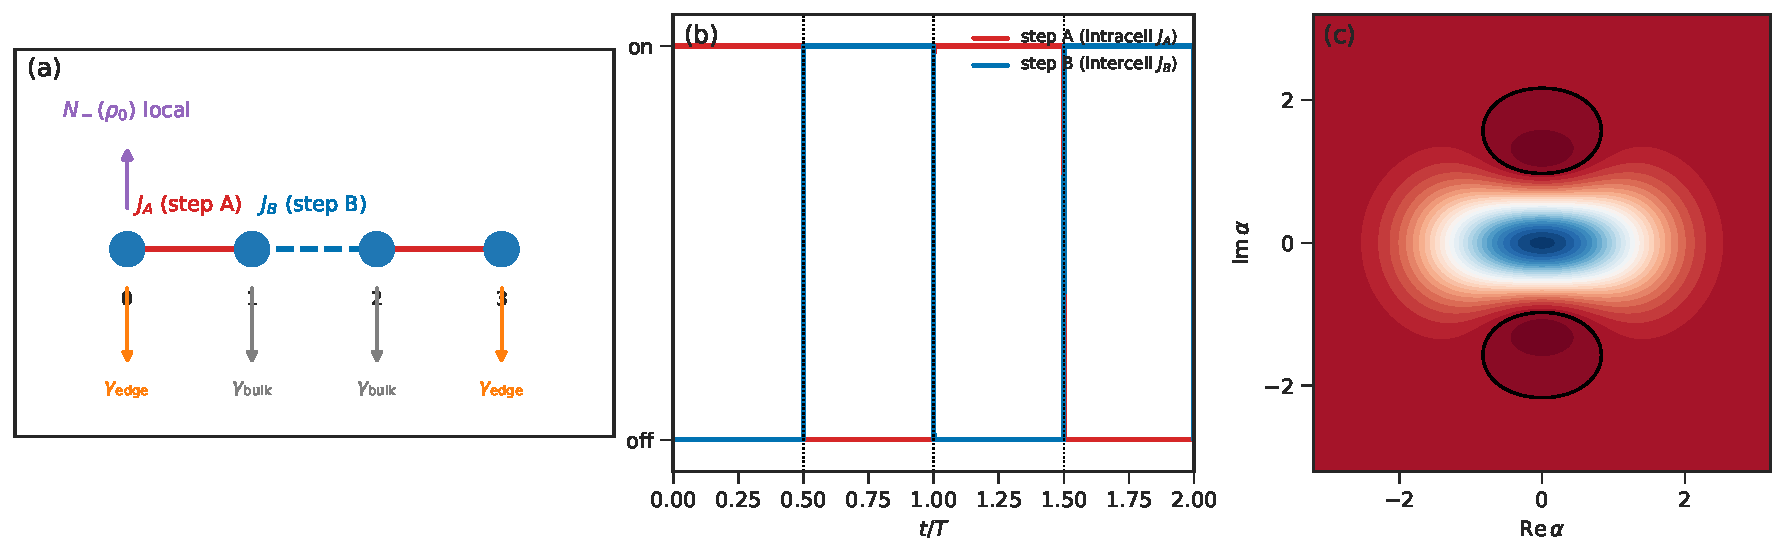
\includegraphics[width=0.98\linewidth]{model_schematic.pdf}
  \caption{Model schematic. (a)~Two-cell chain with intracell ($J_A$, solid) and intercell ($J_B$, dashed) hoppings, edge loss $\gamma_{\rm edge}$ and bulk loss $\gamma_{\rm bulk}$. The tracked quantity is the local Wigner negativity $\Ne$ on the boundary site. (b)~Two-step square drive of period $T=2\pi$. (c)~Even-cat preparation whose local Wigner function is monitored under dissipation.}
  \label{fig:schematic}
\end{figure}

\subsection{Collective edge-mode diagnostic}
\label{sec:edgeobservable}

To test whether any observed contrast is carried by a collective edge mode, we define the Floquet edge vector $u_e(0)$ as the most edge-localized eigenvector of the coherent one-period propagator. Its micromotion-covariant continuation is $u_e(t)=U_{\rm coh}(t)u_e(0)$, and the corresponding mode operator and occupation are
\begin{equation}\label{eq:edge_mode}
  b_e(t)=\sum_j u_{e,j}(t)^*a_j,
  \qquad
  n_e(t)=\braket{b_e^\dagger(t)b_e(t)}.
\end{equation}
In the isolated-mode approximation the occupation would decay as
\begin{equation}\label{eq:passive_reference}
  n_e^{\rm ref}(t)=n_e(0)\exp[-\Gamma_e(t)],
  \qquad
  \Gamma_e(t)=\int_0^t\sum_j\gamma_j|u_{e,j}(s)|^2\,\dd s.
\end{equation}
Equation~\eqref{eq:passive_reference} is exact only for a decoupled passive mode; edge--bulk transfer, Kerr nonlinearity and finite Fock truncation must be bounded separately (see \cref{SI-sec:covariantmethod}).

\section{Results}
\label{sec:results}

We report the local Wigner-negativity contrast between the chiral and trivial sectors under matched dissipation, disorder and system size. The central observation is a sign change with size: the contrast is positive at two unit cells and negative at three, four, and five cells under edge-selective loss, while remaining consistent with zero under uniform loss at zero disorder. In the exact master equation the sign pattern is resolved at two and three cells and directly resolved at four cells ($-\num{0.00032}\pm\num{0.00011}$ at $N_{\rm traj}=\num{200}$), with five cells unresolved; finite-trajectory bias dominates the operational negative branch, so the failure to protect is established at the level of the exact master equation, not of the estimator. Reported contrasts are measured \num{10}-trajectory values rather than converged master-equation values (\cref{SI-sec:trajcount,SI-tab:trajladder}).

\subsection{Size dependence of the local observable (at $t=T$)}
\label{sec:size}

The data comprise \num{4000} matched disorder realizations at two and three cells and \num{16000} at four cells (\num{500}, \num{500}, and \num{2000} per disorder level and loss profile; \cref{SI-sec:statistics,SI-tab:paired-comparison}), plus an independent five-cell extension of \num{300} matched units at $d\le\num{0.5}$ (\cref{SI-sec:size5}). The edge-selective results are summarized in \cref{tab:production}.

\begin{table}[htpb]
\caption{Local Wigner-negativity contrast (chiral $-$ control) under edge-selective loss. Means are taken over matched disorder units; the range spans the four disorder amplitudes (two amplitudes, $N_{\rm MC}=\num{300}$, for the five-cell row). Bootstrap \qty{95}{\percent} intervals at zero disorder are given in the text. Intervals are statistical only and exclude truncation uncertainty (factor-$\sim\num{2}$ magnitude spread at two cells; \cref{SI-tab:nmaxpanel}).}
\label{tab:production}
\begin{ruledtabular}
\begin{tabular}{lcc}
Cells (modes) & $N_{\rm MC}$ & Mean contrast range \\
\hline
\num{2} (\num{4}) & \num{500} & $+\num{0.0131}$ to $+\num{0.0167}$ \\
\num{3} (\num{6}) & \num{500} & $-\num{0.0023}$ to $-\num{0.0020}$ \\
\num{4} (\num{8}) & \num{2000} & $-\num{0.0021}$ to $-\num{0.0018}$ \\
\num{5} (\num{10}) & \num{300} & $-\num{0.0026}$ to $-\num{0.0022}$ \\
\end{tabular}
\end{ruledtabular}
\end{table}

At zero disorder the edge-selective contrast of \eqref{eq:negativity} reads
\begin{align*}
  &\text{\num{4} modes:} & +\num{0.01673} & [\num{0.01565},\,\num{0.01778}],\\
  &\text{\num{6} modes:} & -\num{0.00210} & [\num{-0.00319},\,\num{-0.00100}],\\
  &\text{\num{8} modes:} & -\num{0.00201} & [\num{-0.00255},\,\num{-0.00149}],\\
  &\text{\num{10} modes:} & -\num{0.00218} & [\num{-0.00362},\,\num{-0.00073}].
\end{align*}
The four-mode interval lies entirely above zero; the six-, eight-, and ten-mode intervals lie entirely below zero. The sign change between two and three unit cells is statistically resolved and persists at four and five cells, where the negative branch saturates near \num{0.0021} instead of drifting with size. These are measured values of the \num{10}-trajectory estimator. A trajectory-count ladder validated against the exact master equation at two and three cells places the solver-level negative branch at $\num{9e-5}$--$\num{4e-4}$ in point estimates, with the four-cell sign directly resolved at \num{200} trajectories ($-\num{0.00032}\pm\num{0.00011}$, \qty{95}{\percent} interval excluding zero) and five cells unresolved. The operational negative branch is therefore a property of the estimator, not of the underlying dynamics; the exact master equation confirms the sign change at two and three cells and resolves it at four cells (\cref{SI-sec:trajcount,SI-sec:crosssolver}).

The five-cell value was predicted before measurement. It lies inside its predicted interval (\num{4} of \num{4} conditions: the sign-resolved edge-selective conditions match the predicted sign, the uniform-loss conditions sign-unresolved as predicted; \cref{SI-sec:size5,SI-tab:size5}). The predicted band is wide enough to contain the inverse-size model as well, so its sharp content is the sign match plus the exponential-model proximity (\num{0.08} standard errors) and the exclusion of $1/N$ drift by the measured intervals. The eight-mode contrast, while its bootstrap interval~\cite{Efron1979} excludes zero, exceeds the minimum detectable effect at the attained sample size by a factor of $\approx\num{2.6}$ (observed magnitude $\num{0.00201}$ versus $\Delta_{\min}=\num{0.00077}$ at $N_{\rm MC}=\num{2000}$); the eight-mode result should therefore be interpreted as a small finite-time effect resolved in the current sample, not as a robust or universal signature (see \cref{SI-sec:power}). The local Fock cutoff $N_{\max}=\num{2}$ is low and magnitudes are not converged; the full cutoff panel and its quantitative limitations are given in \cref{SI-tab:nmaxpanel} and \cref{sec:discussion}.

The two-cell signal itself is detected without any grid: on the identical trajectories, displaced Fock-state witnesses of Wigner negativity~\cite{Chabaud2021witnessingwigner}, a grid-free strategy with recent few-copy operational backing~\cite{Chakrabarty2026}, exceed their threshold in \qty{82.4}{\percent} of topological disorder draws versus \qty{10.8}{\percent} for the trivial sector (disjoint Wilson intervals~\cite{Wilson1927}), never under uniform loss and never at the center site (\cref{SI-sec:witness,SI-tab:witness}). Over the same trajectories, the paired relative-entropy non-Gaussianity contrast~\cite{Albarelli2018} is $\num{0.1316}\pm\num{0.0025}$. The witness rates are evaluated at the primary cutoff $N_{\max}=\num{2}$, so ``detected'' refers to a grid-free test at fixed truncation. Joining this witness with the collective-null test draw by draw (\num{10} draws per sector at two cells, $d=\num{0}$) doubly detects \qty{80}{\percent} of topological draws versus \qty{10}{\percent} of trivial draws (\cref{SI-sec:witness}), so the certification does not rest on the collective channel being quiet only in aggregate.

Under uniform loss the contrasts are consistent with zero at $d\le\num{0.5}$ at every size; at stronger disorder the eight-mode contrasts resolve negative offsets of magnitude below $\num{4.2e-4}$, at least four times smaller than the edge-selective contrast at the same disorder (\cref{fig:production}(b)). The same sign pattern remains consistent across all four disorder amplitudes (\cref{fig:robustness}).

\begin{table}[htpb]
  \centering
  \caption{Zero-disorder edge-site negativity $\delta_-$ per sector at $t=T$ under the edge-selective profile ($N_{\max}=\num{2}$, $\num{31}\times\num{31}$ grid). Both sectors start from the identical prepared state with $\delta_-(\num{0})=\num{0.1962}$.}
  \label{tab:sectornegativity}
  \begin{ruledtabular}
  \begin{tabular}{rrrrr}
  Cells (modes) & $N_{\rm MC}$ & Topological & Trivial & Contrast \\
  \hline
  \num{2} (\num{4})  & \num{500}  & \num{0.02368} & \num{0.00695} & $+\num{0.01673}$ \\
  \num{3} (\num{6})  & \num{500}  & \num{0.00478} & \num{0.00688} & $-\num{0.00210}$ \\
  \num{4} (\num{8})  & \num{2000} & \num{0.00466} & \num{0.00667} & $-\num{0.00201}$ \\
  \num{5} (\num{10}) & \num{300}  & \num{0.00508} & \num{0.00725} & $-\num{0.00218}$ \\
  \end{tabular}
  \end{ruledtabular}
\end{table}

The sign change reflects the topological sector rather than growth of the control: within one drive period the topological sector retains only \num{0.02368} of the prepared negativity at two cells (versus $\delta_-(\num{0})=\num{0.1962}$) and drops by a further factor of $\approx\num{5}$ between two and three cells, while the trivial control stays flat at \num{0.0067}--\num{0.0073} across all four sizes (\cref{tab:sectornegativity}).

The same final states, rotated into the collective edge-mode basis, show no collective Wigner negativity in the \num{320} common-site records spanning both Fock truncations ($N_{\max}=\num{2}$ and $\num{3}$) and both system sizes; the \num{240} mode-resolved records remain at or below the truncation floor (maximum \num{1.2e-5}), and the \num{560}-record set is analyzed in \cref{SI-sec:collective-wigner}. The local site-0 contrast instead stays positive at two cells under edge-selective loss (\cref{fig:production}(c)). What is basis-dependent is the marginal Wigner negativity, not the non-Gaussianity itself, which passive rotations preserve; in the tested preparations the negativity appears in the local marginal and not in the collective-mode one. That null is partly built in: the cat-like reference state was prepared on site~0 with only \qty{1.3}{\percent} collective-mode overlap, so its collective marginal starts Gaussian, $\delta_-(\num{0})=\num{0}$ compared with \num{0.1962} for the local site (\cref{SI-tab:collective-null}). The contrast between the two representations is illustrated in \cref{fig:collective-wigner}.

\begin{figure}[htpb]
  \centering
  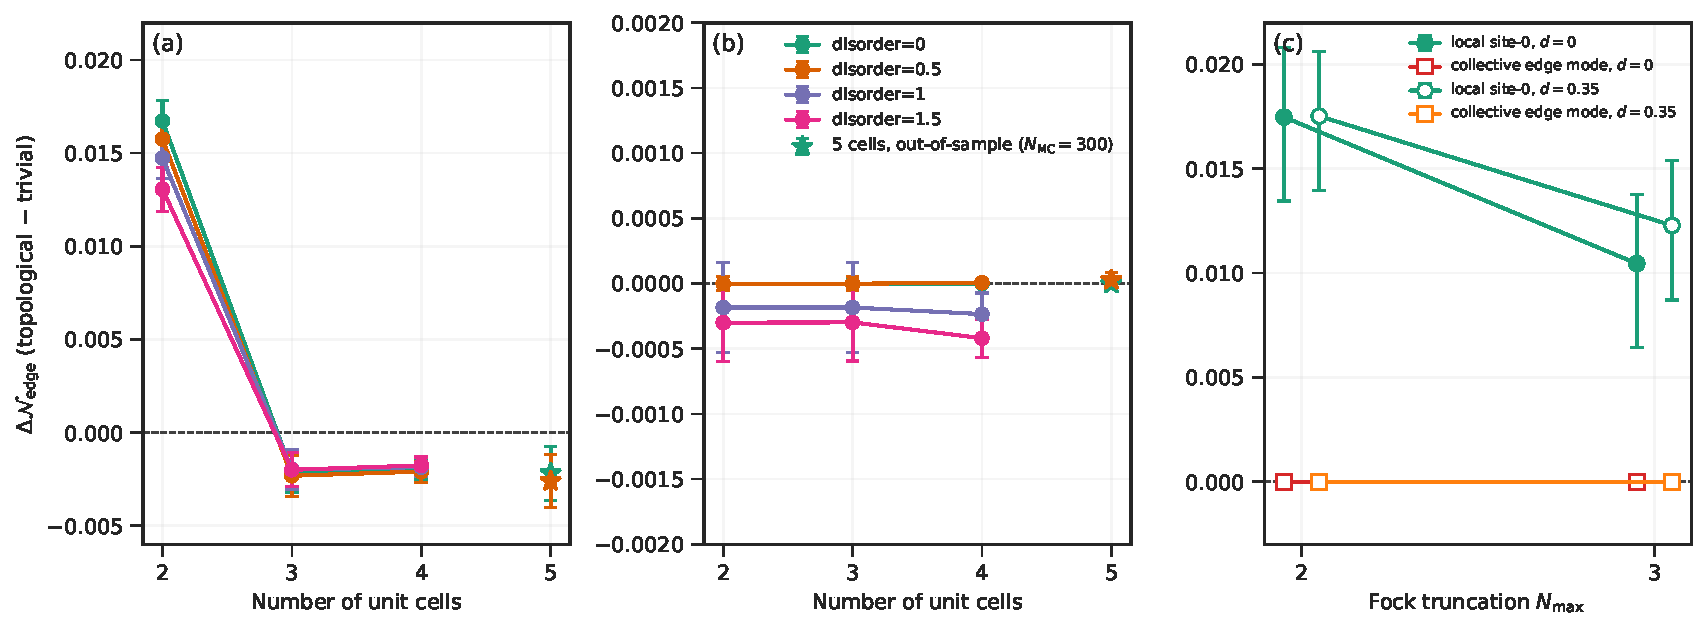
\includegraphics[width=.98\linewidth]{chiral_production_contrast.pdf}
  \caption{Size and loss-profile dependence of the local Wigner-negativity contrast.
  (a)~Edge-selective loss: positive at two cells, negative thereafter; star markers at five cells show the independently predicted point ($N_{\rm MC}=\num{300}$, $d\le\num{0.5}$ only).
  (b)~Uniform loss: consistent with zero at all sizes for $d\le\num{0.5}$; small resolved offsets at stronger disorder.
  (c)~Local site-0 contrast (green circles) versus collective edge-mode contrast (red squares) at two cells; the collective-mode negativity vanishes at both Fock truncations. Filled (open) symbols: $d=\num{0}$ ($d=\num{0.35}$).}
  \label{fig:production}
\end{figure}

\begin{figure}[htpb]
  \centering
  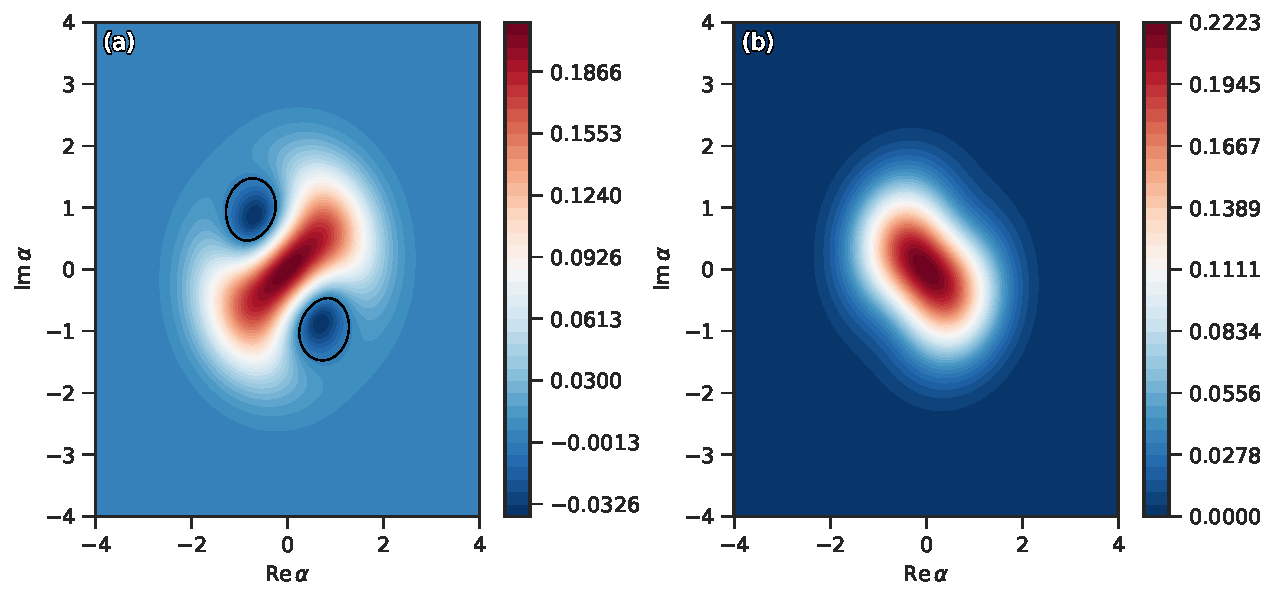
\includegraphics[width=0.8\linewidth]{collective_vs_local_wigner.pdf}
  \caption{Local versus collective-mode Wigner function at two cells under edge-selective loss.
  (a)~Single-site Wigner function on the boundary mode, showing clear negativity.
  (b)~Wigner function of the same final state after rotation into the collective edge-mode basis; the distribution is non-negative.}
  \label{fig:collective-wigner}
\end{figure}

\begin{figure}[htpb]
  \centering
  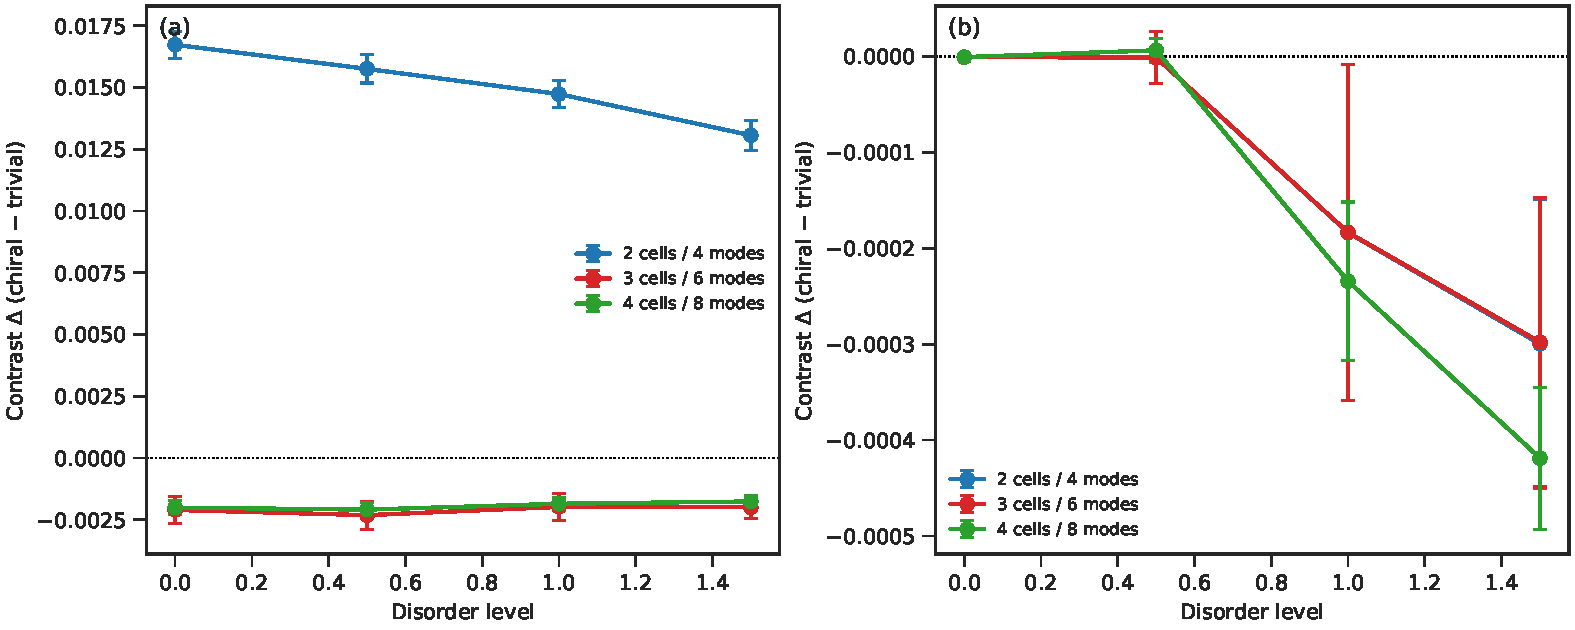
\includegraphics[width=0.8\linewidth]{robustness_matrix.pdf}
  \caption{Disorder robustness of the local contrast.
  (a)~Edge-selective loss: the sign pattern is stable across all four disorder amplitudes.
  (b)~Uniform loss: all values remain near zero.
  Error bars are standard errors of the matched contrast.}
  \label{fig:robustness}
\end{figure}

\subsection{Dependence on the bulk invariant}
\label{sec:invariantsweep}

The discriminating test posed in the Introduction asks whether the local contrast follows the bulk invariant, which changes at a gap closing, or the edge-mode localization, which varies continuously. A dimerization scan along $J_A+J_B=\num{1.3}$ (\num{19} points with $J_A$ from \num{0.1} to \num{1.2}, two and three cells, $N_{\rm MC}=\num{500}$ realizations per point at $d=\num{0}$ and \num{0.35}, disorder draws and trajectory seeds shared across points) crosses all three gap closings of the model. The sweep observable is the edge-minus-center negativity at each dimerization point; because the center-site negativity vanishes identically on this grid it equals the edge negativity itself, and it is not the matched topological-minus-trivial sector contrast of \cref{tab:production}, only the difference between the two dimerization endpoints maps onto that sector contrast. Continuity across closings is therefore a property of the sweep observable; its implication for the sector contrast rests on the endpoint differences.

This observable is non-monotone: it peaks inside the strongly dimerized topological regime ($+\num{0.05928}$ at two cells, $J_A=\num{0.20}$), is zero to within \num{2e-5} over $\num{0.6}\le J_A\le\num{0.8}$, a window containing the $\nu_0=-1\to0$ transition and points gapped on both sides, and becomes finite again in the strongly dimerized trivial regime. At each closing the contrast is continuous with its bracketing points on matched draws (largest residual $+\num{0.00086}\pm\num{0.00017}$, \qty{1.95}{\percent} of the local signal and below the two-cell $\Delta_{\min}=\num{0.001543}$ at $N_{\rm MC}=\num{500}$), and the difference between the two dimerization endpoints reproduces the primary sign pattern ($+\num{0.01673}$ and $-\num{0.00189}$ against $+\num{0.01673}$ and $-\num{0.00210}$). The local contrast therefore does not follow the bulk invariant. It is significantly anti-correlated with the measured edge-mode localization length at two cells (Pearson $r=\num{-0.680}$, $p=\num{0.0013}$), with the same but unresolved trend at three cells (\cref{SI-sec:dimerization,SI-tab:dimerization}); of the two alternatives posed in the Introduction, the local contrast follows neither exactly, but its residual size dependence is better accounted for by the measured localization length than by the invariant.

\subsection{Micromotion-covariant edge mode}
\label{sec:covariant}

When the edge occupation is evaluated in the micromotion-covariant frame (\cref{eq:edge_mode}), the common-site passive contrast drops to \num{3.88e-4} [\num{3.58e-4},\,\num{4.18e-4}] (mean and \qty{95}{\percent} interval) while the mode-resolved preparation yields a small negative value \num{-1.59e-5} [\num{-1.82e-5},\,\num{-1.36e-5}]. The maximum residual relative to the isolated-mode reference (\cref{eq:passive_reference}) reaches \num{0.0396} (common-site) and \num{0.3826} (mode-resolved), factors of \num{40} and \num{380} above the stated \num{1e-3} residual threshold. The micromotion correction eliminates a frame ambiguity, yet the passive survival reference itself is not recovered (\cref{fig:covariant}; see also \cref{SI-sec:covariantmethod}).

The residuals are diagnostic discrepancies, not numerical-error estimates, and this analysis does not establish a topology-by-loss mechanism.

\begin{figure}[htpb]
  \centering
  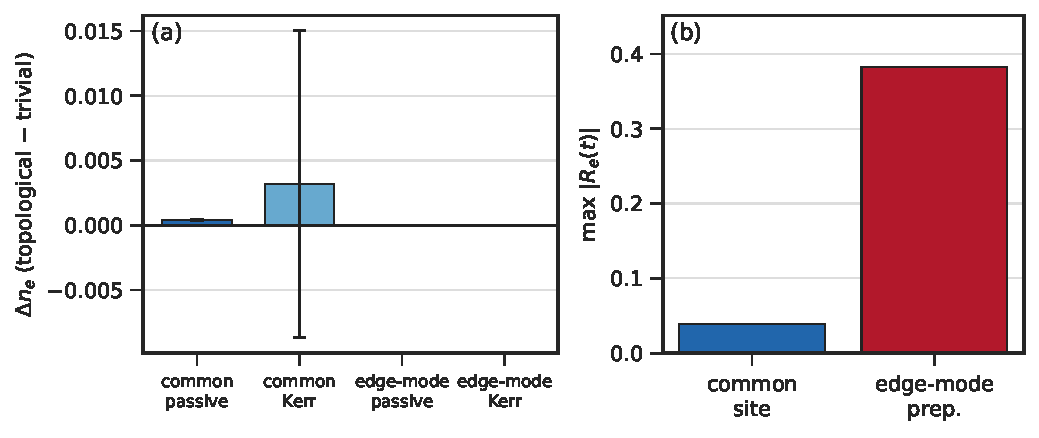
\includegraphics[width=0.8\linewidth]{edge_mode_covariant_summary.pdf}
  \caption{Micromotion-covariant edge-mode analysis. (a)~Matched edge-population contrasts at zero disorder and edge-selective loss for the two preparations and two Kerr conditions. (b)~Maximum residual of the conditional passive reference.}
  \label{fig:covariant}
\end{figure}

\subsection{Deterministic controls and finite-size mechanism}
\label{sec:controls}

Two exactly solvable benchmarks isolate kinematic and dissipative effects. In the absence of loss and Kerr nonlinearity the covariant edge population remains unity to machine precision ($1-p_e(t)<\num{1.4e-15}$), while the laboratory-frame population falls to $\approx\num{0.895}$. Under uniform loss the integrated-exposure reference is recovered to \num{1.94e-15}; under the edge-selective profile a residual of order \num{1e-3} appears, consistent with weak edge--bulk mixing during micromotion. These controls validate the implementation of the observable and quantify a finite-size correction; they do not by themselves imply protection of a non-Gaussian resource (detailed derivations and decompositions appear in \cref{SI-sec:unitarybenchmark}).

The underlying finite-size mechanism is summarized in \cref{fig:mechanism}: the edge-mode observable departs from the isolated-mode prediction as the chain and loss profile change, and the jump in edge--bulk participation between two and three cells correlates with the observed sign change of the local contrast. The empirical bulk-participation diagnostic and two-photon dwell analysis behind panels (b) and (c) are given in \cref{SI-sec:localizer-transfer} (\cref{SI-tab:bound-verification,SI-tab:closedform-kappa}); neither constitutes a general open-system decay theorem.

\begin{figure}[thpb]
  \centering
  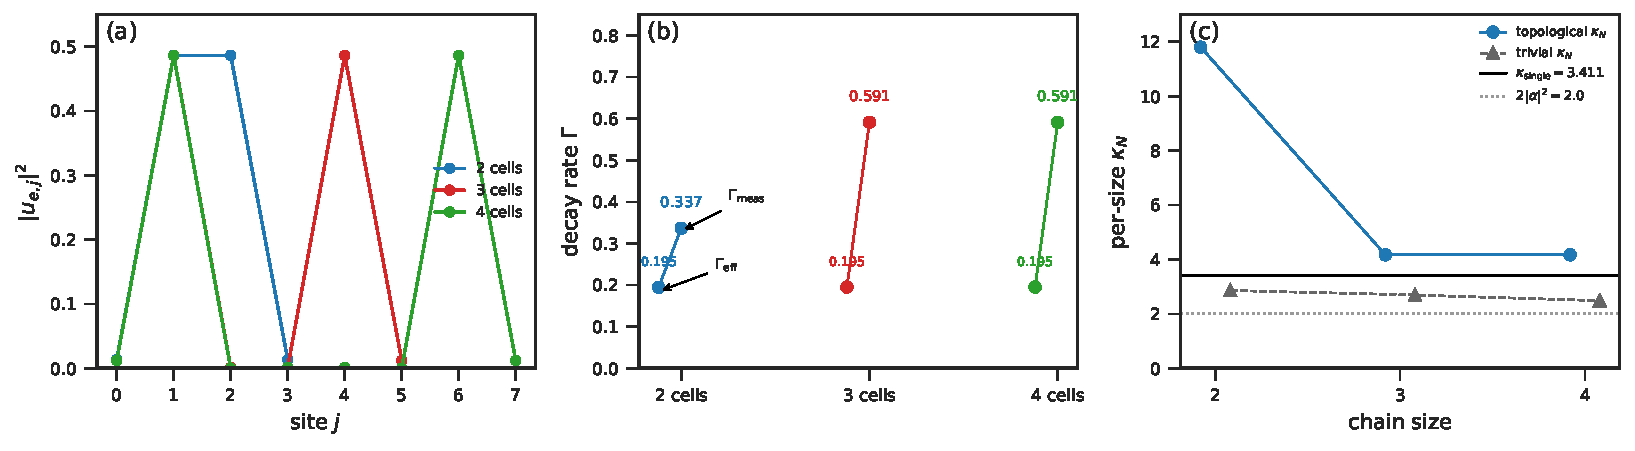
\includegraphics[width=.98\linewidth]{mechanism_panel.pdf}
  \caption{Finite-size mechanism diagnostics.
  (a)~Edge-mode weight $|u_{e,j}|^2$ for chains of two, three and four unit cells, showing progressive delocalization.
  (b)~Measured decay rate $\Gamma_{\rm meas}$ compared with the isolated-mode prediction.
  (c)~Size-dependent prefactor $\kappa_N$ extracted from the two-photon dwell time (horizontal line: single-site reference $\kappa=\num{3.411}$).}
  \label{fig:mechanism}
\end{figure}

\section{Discussion}
\label{sec:discussion}

The coherent two-step model supports well-defined integer Floquet sectors with open quasienergy gaps and the expected finite-chain edge modes~\cite{Asboth2014}. That statement concerns only the single-particle backbone. Once the system is opened to a structured bath and a local Kerr nonlinearity is retained, a nonlinear observable, the integrated Wigner negativity, can change sign with system size and vanish under uniform loss while the coherent classification remains unchanged. This separation is the central result: a bulk Floquet invariant does not automatically protect a finite-time non-Gaussian resource. The comparison is direct: across a dimerization sweep that crosses all three gap closings the contrast changes continuously and vanishes on a window that straddles the topological transition (\cref{sec:invariantsweep}).

The size dependence under the edge-selective profile is resolved and reproducible across disorder amplitudes up to \num{1.5} (\cref{fig:robustness}). The conditional passive reference fails its stated residual budget (\cref{SI-sec:covariantmethod}), so the sign change is a reproducible finite-time observation rather than a confirmed mechanism. The independently predicted five-cell size reinforces the finite-size reading: predicted from the three smaller sizes before measurement, the ten-mode contrast lands inside its predicted interval at $-\num{0.00218}$ (\cref{SI-sec:size5}), extending the negative branch to five cells; the measured intervals exclude the inverse-size prediction ($-\num{0.0088}$), ruling out an inverse-size drift even though that point lies inside the predicted ensemble band. Under uniform loss the contrast falls to the \num{1e-6} level at zero disorder at every size. This shows the positive small-system signal exists only for a sharply structured loss profile ($\gamma_{\rm edge}/\gamma_{\rm bulk}=\num{5e-4}$); the signal is lost once the ratio reaches \num{0.5}. At the intermediate ratio \num{1e-2} the two-cell contrast persists at $+\num{0.0158}$ (budget-matched $+\num{0.0156}$ at $d=\num{0}$; \cref{SI-tab:lossratio}). This dependence survives when the total loss budget is held fixed at the primary value (\cref{SI-tab:lossratio,SI-sec:lossratio}). This extreme sensitivity shows that bath engineering matters as much as Hamiltonian engineering. The negative branch would be retracted by a solver-level positive at three or four cells or by a sign reversal under doubled trajectories; neither has occurred.

Both directions already have demonstrated experimental primitives: parity-based direct Wigner reconstruction~\cite{Lutterbach1997}, macroscopic cavity cat states in circuit QED~\cite{Vlastakis2013}, and dissipatively stabilized quantum manifolds~\cite{Touzard2018}, with a standard homodyne-based measurement chain on the optomechanical side~\cite{Aspelmeyer2014}; the resulting measurement overhead for these observables is summarized in \cref{SI-sec:hardware}. Cast as an experimental prediction, the two-cell witness asymmetry is the near-term target: \qty{82.4}{\percent} versus \qty{10.8}{\percent} single-shot certification rates separate the sectors in a few hundred displaced photon-counting repetitions with no tomography, while the full sign pattern is a tomography-level prediction at sub-$\num{1e-3}$ resolution (\cref{SI-sec:witness,SI-tab:testable}); the step-by-step protocol, with shot budgets and acceptance criteria, is summarized in \cref{SI-sec:measurement-protocol}.

The primary ratio is deliberately extreme: no existing bosonic lattice platform provides a $\num{2000}\colon\num{1}$ loss ratio between neighboring sites, so the positive four-mode signal defines a theoretical boundary condition rather than a realistic device scenario.

Projection onto the collective edge mode yields a numerical null result: no resolved edge-mode Wigner negativity is observed in the \num{560} matched records examined (\cref{SI-sec:collective-wigner}). This null must be read with its preparation geometry: the cat-like reference state was prepared on site~0, overlapping the collective edge mode by only \qty{1.3}{\percent}, and its collective marginal already starts Gaussian, so the absence of collective negativity is partly built into the tested preparation rather than discovered in it. The null is therefore a property of the tested preparation, not a theorem about collective-mode negativity. What the comparison does show is that the marginal negativity of these trajectories lives in the site basis, while the non-Gaussianity itself is invariant under the passive rotation and is not located in any basis (\cref{SI-tab:collective-null}). The micromotion-covariant occupation analysis reaches the same conclusion: weak edge--bulk mixing during the drive invalidates the simplest protection argument. While accounting for micromotion in Floquet observables is well established~\cite{Xu2022micromotion} and open Floquet physics is increasingly recognized~\cite{Mori2023,Chen2024,Roy2025}, these ingredients alone do not guarantee protection of local Wigner negativity.

These findings sit naturally within the emerging mixed-state SPT framework~\cite{Paszko2024,Chirame2025}, where mixed-state topological diagnostics at nonzero temperature are by now well developed~\cite{Hannukainen2026} and include a holographic bulk-boundary view~\cite{Sun2025holographic}. That framework itself has sharp limits: steady-state mixed SPT order is unstable to generic symmetric perturbations via strong-to-weak spontaneous symmetry breaking~\cite{Shah2025instability}. Recent work has established that certain topological features of a mixed state can survive broad classes of local noise even when the underlying edge modes are not themselves protected. The present results supply the complementary negative statement for a nonlinear, finite-time observable: kinematic edge modes and a favorable loss profile do not, by themselves, guarantee protection of local Wigner negativity. The distinction is consequential. Mixed-state SPT order constrains steady-state properties and symmetry charge; the quantity tracked here is a transient, basis-dependent functional of a driven dissipative trajectory.

Related work on driven-dissipative topological systems has focused primarily on the engineering of topological steady states~\cite{Diehl2011,Bardyn2013}, on driven-dissipative topological phases in parametric resonator arrays~\cite{GomezLeon2023resonator}, and on the interplay of nonlinearity with topological transport~\cite{Peano2016}. Static dissipation has been demonstrated to stabilize Floquet quasienergy states in experiment and topological pumping in numerics~\cite{Ritter2025autonomous}. Protected long-range order has indeed been reported for the steady-state correlations of driven-dissipative bosonic chains~\cite{ClaveroRubio2026}, and Wigner negativity itself can be stabilized at steady state by parity engineering rather than by topology~\cite{Liu2026} or generated by single-mode Kerr dynamics under weak loss with no topological structure involved~\cite{Raza2026}; none of these protects a transient trajectory functional such as the one tracked here. The present results address a complementary question: the fate of a transient non-Gaussian resource under a pre-existing coherent Floquet classification and structured loss.

\begin{table}[htpb]
  \centering
  \caption{Boundary matrix for topological claims on observables in driven bosonic lattices. Entries summarize what is established in the literature for each cell and what the present work tests; references are given in the text. Quoted contrasts are measured \num{10}-trajectory values throughout; the solver-level ladder is exact at two and three cells, resolved at four, and pending at five.}
  \label{tab:boundary}
  \begin{ruledtabular}
  \begin{tabular}{>{\raggedright\arraybackslash}p{0.26\linewidth}>{\raggedright\arraybackslash}p{0.32\linewidth}>{\raggedright\arraybackslash}p{0.32\linewidth}}
  Dissipator structure & Linear, Gaussian, or steady-state observable & Nonlinear transient resource (finite window) \\
  \hline
  Generic (symmetry-breaking) loss & Enhanced or transported in specific platforms~\cite{Li2024photonblockade,Perez2024domainwalls} & Not protected (this work) \\
  Symmetry-respecting or engineered loss & Protected or metastable under additional symmetry conditions~\cite{Diehl2011,Bardyn2013,YanayClerk2018,Paszko2024,Chirame2025} & Tested here and not protected: small negative contrast with no sign change across sizes, though the profile also erases the sector distinction (\cref{SI-sec:chiral-loss}) \\
  Closed-system / kinematic Floquet features & Resilient edge populations under timing noise; edge states at Floquet criticality~\cite{Bhargava2025,Zhou2025Floquet} & No transfer to dissipative trajectory functionals tested or assumed (this work) \\
  \end{tabular}
  \end{ruledtabular}
\end{table}

Several works report topological preservation of nonclassical correlations or their enhancement~\cite{Wang2019Optica,Perez2024domainwalls,Li2024photonblockade}. These observations and the present negative result are complementary rather than contradictory. The reported protection concerns correlation or blockade observables in their respective operating regimes, and for entangled non-Gaussian two-photon states it weakens as the entanglement grows~\cite{Tschernig2021}; the resource tracked here instead is a transient local functional generated by a strong Kerr interaction under a deliberately extreme loss profile, and the quantity tested is the matched topological-minus-trivial contrast rather than the absolute survival of the resource. Our results therefore exclude the inference from a bulk invariant to a protected non-Gaussian resource in this regime; they do not dispute the preservation of correlations in the settings where it has been measured.

Topology can also protect a local metrological quantity, and the contrast with the present case is instructive: in an open Kitaev chain a Majorana zero mode fixes the boundary quantum Fisher information at a nonzero plateau for times exponentially long in system size~\cite{Plodzien2026}. That protection relies on a quadratic, undriven, parity-preserving setting with a symmetry-protected localized mode; the present driven, nonlinear, finite-time non-Gaussian resource does not inherit it, which is precisely the boundary this study maps.

Our results suggest three operational conditions under which a bulk invariant could constrain a local non-Gaussian resource:
\begin{enumerate}
  \item a dissipator that respects the protecting symmetry;
  \item an observable supported on the protected mode's basis; and
  \item a mode localization that is stable across the tested sizes.
\end{enumerate}
That the spatial pattern of dissipation matters for edge dynamics is supported by trajectory-resolved studies of monitored SSH chains, where shielding the chain edges from loss recovers unitary-like edge-mode features~\cite{Salatino2025}. These are conjectures offered for future tests, not established criteria; the present data satisfy none of them.

The first is tested and fails: loss confined to one sublattice, so that every collapse operator commutes with the chiral operator, leaves a small resolved negative contrast ($-\num{0.00081}\pm\num{0.00005}$ at two cells, statistically unchanged at $-\num{0.00079}\pm\num{0.00009}$ once the total loss budget and the edge-to-bulk rate ratio are matched to the control; \cref{SI-sec:chiral-loss,SI-tab:chiralloss}). Under this profile the two sectors retain nearly the same edge negativity (topological \num{0.02285} versus trivial \num{0.02366} at two cells, $d=\num{0}$). So the profile erases the sector distinction rather than isolating a protection mechanism, and the residual contrast is that of two nearly indistinguishable states. This failure is specific to the observable class tested here: weak symmetries alone have been shown to protect quantized topological responses of string-order diagnostics in one-dimensional mixed states~\cite{Huang2025weaksymmetries}, so for nonlinear transient observables the frontier between protected and unprotected lies in the observable as much as in the symmetry. The second and third are violated by construction: the resource is a site-basis quantity whose projection onto the protected mode basis returns a null (\cref{SI-sec:collective-wigner}), and the sign changes with size. Whether some other combination of these conjectured conditions suffices remains the natural next test: a symmetry-respecting dissipator at an intermediate loss ratio (two cells), a mode-basis non-Gaussian observable at fixed truncation, and a size ladder at matched budget.

To reconcile this sensitivity with topological theory, future analyses seeking such a connection will need local, energy-resolved diagnostics such as the spectral localizer~\cite{CerjanLoring2025Tutorial, WongCerjanCole2024Quantitative} and local Floquet invariants~\cite{Ghosh2024Local}. The localizer bound established here for the coherent single-particle model (\cref{SI-sec:localizer}) does not extend to the open nonlinear generator: the Wigner negativity is a many-body functional of the full Lindblad trajectory, and no transfer theorem connects the localizer gap to its protection.

Several limitations bound the scope of our claim. All parameters are normalized; we assert no device-specific mapping and infer no compatibility with any specific cQED device~\cite{Blais2021Circuit} (see \cref{SI-sec:hardware} for scale comparisons). The local Fock cutoff $N_{\max}=\num{2}$ is low; no tested cutoff resolves a sign opposite to the primary pattern (up to $N_{\max}=\num{4}$ at all three tested sizes; \cref{SI-sec:nmaxpanel,SI-tab:nmaxpanel}). Although the three-cell $N_{\max}=\num{4}$ entry is itself unresolved against zero ($-\num{0.0012}\pm\num{0.0025}$), the four-cell $N_{\max}=\num{4}$ entry clears zero only marginally ($-\num{0.0017}\pm\num{0.0016}$), and the five-cell out-of-sample point was run at $N_{\max}=\num{2}$ only. Absolute magnitudes stay cutoff-sensitive: at two cells the magnitude is non-monotone with a $\approx\num{2}\times$ spread across the tested cutoffs (\num{0.0113}--\num{0.0250}) and the paired $N_{\max}=\num{2}\to\num{3}$ zero-disorder shift excludes zero ($-\num{0.00540}$, a factor \num{1.48} reduction). At three and four cells the same shift is consistent with zero, as is the paired $N_{\max}=\num{2}\to\num{4}$ shift at four cells ($+\num{0.0004}\pm\num{0.0010}$); no magnitude is claimed cutoff-converged. No tested cutoff reverses the sign, and no tested cutoff resolves a sign opposite to the primary pattern.

Detection margins over the minimum detectable effect are modest: $\approx\num{1.3}\times$ at six modes, $\approx\num{2.6}\times$ at eight modes ($N_{\rm MC}=\num{2000}$), and $\approx\num{1.05}\times$ at the independently predicted five-cell point (\cref{SI-sec:power}), so these are small finite-time effects rather than robust signatures.

The trivial sector control has a different edge-mode structure; a random-hopping chain with the same loss profile would provide a cleaner null, but that comparison remains beyond the present scope. A Kerr-free primary stratum, run in full, separates filtering of the prepared negativity from interaction-generated effects: the sign pattern and the uniform-loss null are unchanged at $\chi=0$, and the exact two-cell contrast falls from \num{0.022328} to \num{0.010467} (a factor \num{2.1}), so the nonlinearity amplifies rather than creates the sector contrast (\cref{SI-sec:kerrfree,SI-tab:kerrfree}). The tracked contrast is thus filtered prepared negativity, not a generated many-body resource, which is why the failure claim concerns protection, not production.

The finite-trajectory estimator itself carries a bias: because the negativity is a nonlinear functional of the trajectory-averaged state, the \num{10}-trajectory primary estimator overestimates the near-zero sector negativities and contributes $\sim\num{2e-3}$ to the negative branch. A trajectory-count ladder validated against the exact master equation at two and three cells corrects for this (solver-level resolution as stated in \cref{sec:results}; \cref{SI-sec:trajcount,SI-tab:trajladder}). The same ladder at two and four periods resolves the small $2T$ reversal as an estimator artefact and brackets the $4T$ revival against the exact value (\cref{SI-sec:trajcount}), so the reported contrasts are measured \num{10}-trajectory values rather than converged master-equation values.

The single-period data capture a dynamical snapshot: a multi-period scan shows the two-cell contrast vanishes at $2T$ and revives at $4T$--$8T$ (\cref{SI-tab:multiperiod}), tracking the topological-sector edge population survival; this revival does not occur at three cells, reinforcing the size-specific interpretation. A \num{64}-period stroboscopic extension extends this picture: the two-cell branch reaches its largest value at $4T$ ($+\num{0.0772}\pm\num{0.0026}$) and, at $d=\num{0}$, the numerical floor by ${\approx}\num{37}T$, and the three-cell negative branch never becomes significantly positive at any of the \num{64} periods at $d\le\num{1}$, although at $d=\num{1.5}$ a negative contrast grows in both loss profiles by $64T$, so the uniform-loss null is a $t=T$ statement at that disorder level (\cref{SI-sec:longtime,SI-tab:longtime}). Stroboscopic $t=T$ is the comparison point because the sector classification itself is defined at integer periods.

Within a single period the dependence is stronger still: sampled at nine phases of the drive the contrast swings by an order of magnitude and changes sign under every tested condition, and the uniform-loss null holds only at $t=T$ (\cref{SI-sec:micromotion,SI-tab:micromotion}), so the reported values are conditional on stroboscopic sampling.

Finally, the edge-selective profile is deliberately extreme. Together these restrictions define a precise boundary condition: any future claim of topological protection for a non-Gaussian resource in a driven bosonic chain must demonstrate size-robustness, basis-independence, and survival under less idealized dissipation~\cite{Sieberer2025}; the supporting diagnostics are compiled in \cref{SI-sec:convergence,SI-tab:scope-limitations}.

\section{Conclusion}
\label{sec:conclusion}

We examined a chiral Floquet SSH backbone to determine whether its distinct coherent sectors leave a finite-time imprint on a dissipative non-Gaussian observable. The local Wigner-negativity contrast changes sign between two and three cells, a pattern resolved in the exact master equation at two and three cells, directly resolved at four cells, and resting on extrapolation at five cells (\cref{SI-sec:crosssolver}), and varies continuously through all three gap closings of a dimerization sweep instead of tracking the bulk invariant. It is not restored by dissipation that commutes with the chiral operator at a matched budget, and it changes sign with the phase of the drive at which it is sampled. Beyond the single result, the study provides three transferable elements for protection claims on driven-dissipative resources: a prediction fixed before measurement (\cref{SI-sec:size5}), a boundary matrix locating each claim against the literature (\cref{tab:boundary}), and a grid-free witness chain that reduces the central effect to a few-hundred-shot measurement (\cref{SI-sec:witness,SI-tab:testable}).

Displaced Fock-state witnesses detect the two-cell negativity without a phase-space grid on the identical trajectories, whereas a collective-mode analysis of the tested conditions, including a cat-like reference state prepared with only \qty{1.3}{\percent} collective-mode overlap, resolves no edge-mode negativity. Over \num{64} periods, the two-cell branch reaches the numerical floor by ${\approx}\num{37}T$ at $d=\num{0}$ and the three-cell branch decays to the floor at $d\le\num{1}$, with a single small estimator-level reversal of the two-cell branch at \num{2}$T$ (\cref{SI-tab:longtime}). These findings establish a reproducible finite-size and loss-profile sensitivity, not topological protection: a coherent bulk invariant cannot by itself guarantee protection of nonlinear mixed-state observables. The work defines a falsifiable boundary condition for future open-system Floquet resource studies and shows that the observable of interest must be validated directly rather than inferred from coherent-sector topology alone.

\section*{Supplemental Material}

See Supplemental Material at [URL will be inserted by publisher] for the model equations, solver settings, matched-analysis and uncertainty details, convergence diagnostics, the collective-mode Wigner analysis, and the deterministic controls underlying the main text.

\section*{Data availability}

The data that support the findings of this study are available within the article and its Supplemental Material. Manuscript sources, deterministic analysis scripts, and the environment specification are publicly archived at \url{https://github.com/NanaEngo/floquet-topology-synthetic-flux}.

\section*{Acknowledgments}

We thank the Stellenbosch Institute for Advanced Study for hospitality. Computational resources were provided by the penavoraserver cluster (ThinkStation P720, 128 GB RAM, 48 cores) through Penabei Samafou; supporting data are provided with the manuscript. This work received no external funding.

\section*{Author contributions}

JD and PD performed the numerical simulations and analyzed the data. AHAA, AE, NM contributed to the theoretical framework and provided critical feedback on the results. SGNE conceived and supervised the project, directed the research. PD and SGNE wrote the final version of the manuscript. All authors reviewed and approved the final manuscript.

\section*{Competing interests}

The authors declare no competing interests.

\section*{Use of AI}

AI-based language models were used to support literature searches, to refine and debug analysis scripts, and to check DOIs and bibliographic information. All AI-generated content was verified and edited by the authors, who remain fully responsible for the manuscript. All authors remain responsible for the accuracy, originality, interpretation, and final wording of this manuscript.

\bibliographystyle{apsrev4-2}
\bibliography{references}

\end{document}
